\documentclass{article}

% Language setting
% Replace `english' with e.g. `spanish' to change the document language
\usepackage[spanish]{babel}

% Set page size and margins
% Replace `letterpaper' with `a4paper' for UK/EU standard size
\usepackage[letterpaper,top=2cm,bottom=2cm,left=3cm,right=3cm,marginparwidth=1.75cm]{geometry}

% Useful packages
\usepackage{amsmath}
\usepackage{graphicx}
\usepackage{enumitem}
\usepackage{comment}
\usepackage{wrapfig}
\usepackage[colorlinks=true, allcolors=blue]{hyperref}

\title{Matemática Discreta Tema 2. Combinatoria}
\author{Martín González Dios 
\href{https://github.com/martindios}{\includegraphics[height=0.5cm]{github.png}}}

\begin{document}
\maketitle

\section{Principios básicos de conteo}
Sea $A$ un conjunto finito. $|A|$ = cardinal de $A$ (número de elementos del conjunto)
\subsection{Principio de adición (suma)}
\textbf{Sean $A$ y $B$ dos conjuntos disjuntos ($A$ $\cap$ $B$ = $\emptyset$), entonces $|A \cup B|$ = $|A|$ + $|B|$} \\
Sean $A_1, A_2, ..., A_n$ conjuntos disjuntos 2 a 2, entonces $|A_1 \cup A_2 \cup ...  \cup A_n|$ = $|A_1|+|A_2|+...+|A_n|$ \\

\textbf{Ejemplo}: Supongamos que se elige como representante para un comité universitario a un miembro de la facultad de matemáticas o a un estudiante que es un major en matemáticas. ¿Cuántas elecciones diferentes hay para este representante si hay 37 miembros de la facultad de matemáticas y 83 majors en matemáticas, y nadie es tanto miembro de la facultad como estudiante? \\

Hay 37 maneras de elegir a un miembro de la facultad de matemáticas y hay 83 maneras de elegir a un estudiante que es un major en matemáticas. Elegir a un miembro de la facultad de matemáticas nunca es lo mismo que elegir a un estudiante que es un major en matemáticas porque nadie es tanto miembro de la facultad como estudiante. Por la regla de la suma, se sigue que hay $37 + 83 = 120$ maneras posibles de elegir a este representante.\\

Podemos \textbf{extender la regla de la suma} a más de dos tareas. Supongamos que una tarea se puede realizar de una de $n_1$ maneras, de una de $n_2$ maneras, \ldots, o de una de $n_m$ maneras, donde ninguno de los conjuntos de $n_i$ maneras de realizar la tarea es el mismo que ninguno de los conjuntos de $n_j$ maneras, para todos los pares $i$ y $j$ con $1 \leq i < j \leq m$. Entonces, el número de maneras de realizar la tarea es $n_1 + n_2 + \cdots + n_m$. Esta versión extendida de la regla de la suma es a menudo útil en problemas de conteo.

\newpage

\subsection{Principio de la diferencia}
Sea $U$ el conjunto “universo”, $A$ un conjunto y $\overline{A}$ su complementario ($A \cap \overline{A} = \emptyset$ y $A \cup \overline{A}$ = $U$), entonces $|\overline{A}| = |U| - |A|$ \\
\textbf{Ejemplo}: ¿Cuántas cadenas de bits de longitud ocho comienzan con un bit 1 o terminan con los dos bits 00? \\

\begin{wrapfigure}[]{r}{0.18\linewidth}
    \centering
    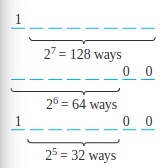
\includegraphics[width=\linewidth]{img-t2/img_192_46.png}
\end{wrapfigure}

Podemos construir una cadena de bits de longitud ocho que comience con un bit 1 o que termine con los dos bits 00. Podemos construir una cadena de bits de longitud ocho que comience con un 1 de $2^7$=128 maneras. Esto se sigue de la regla del producto (siguiente punto), porque el primer bit se puede elegir de una sola manera y cada uno de los otros siete bits se puede elegir de dos maneras. De manera similar, podemos construir una cadena de bits de longitud ocho que termine con los dos bits 00, de $2^6$=64 maneras. Esto se sigue de la regla del producto, porque cada uno de los primeros seis bits se puede elegir de dos maneras y los últimos dos bits se pueden elegir de una sola manera.\\

Algunas de las maneras de construir una cadena de bits de longitud ocho que comienza con un 1 son las mismas que las maneras de construir una cadena de bits de longitud ocho que termina con los dos bits 00. Hay $2^5$=32 maneras de construir tal cadena. Esto se sigue de la regla del producto, porque el primer bit se puede elegir de una sola manera, cada uno de los bits del segundo al sexto se puede elegir de dos maneras, y los últimos dos bits se pueden elegir de una manera. \\

En consecuencia, el número de cadenas de bits de longitud ocho que comienzan con un 1 o terminan con 00, que es igual al número de maneras de construir una cadena de bits de longitud ocho que comienza con un 1 o que termina con 00, es $128+64-32=160$.

\subsection{Principio de la multiplicación (producto)}
Sean $A$ y $B$ dos conjuntos finitos $|A \times B|$ = $|A| \cdot |B| \neq |B \times A|$ (mismo cardinal, distintos elementos). \\
Sean $A_1, A_2, ..., A_n$ conjuntos $\xrightarrow{} |A_1 \times A_2 \times ... \times A_n|$ = $|A_1| \cdot |A_2| \cdot ... \cdot |A_n|$ \\

\textbf{Ejemplo}: ¿Cuántas matrículas diferentes se pueden hacer si cada matrícula contiene una secuencia de tres letras mayúsculas en inglés seguidas de tres dígitos (y no se prohíben las secuencias de letras, incluso si son obscenas)? \\

Hay 26 opciones para cada una de las tres letras mayúsculas en inglés y diez opciones para cada uno de los tres dígitos. Por lo tanto, mediante la regla del producto, hay un total de $26 \cdot 26 \cdot 26 \cdot 10 \cdot 10 \cdot 10$ = 17,576,000 matrículas posibles.

\subsection{Principio de la biyección}
Sean $A$ y $B$ conjuntos finitos y sea f: $A \xrightarrow{} B$ una aplicación biyectiva, entonces $|A|$ = $|B|$

\newpage

\subsection{Principio del palomar}
Si hay n+1 palomas (objetos) y n nidos (cajas), algún nido contendrá al menos $\lceil n/k \rceil$ palomas. \\

\textbf{Ejemplo}: ¿Cuántas cartas deben seleccionarse de una baraja estándar de 52 cartas para garantizar que al menos tres cartas del mismo palo sean elegidas? ¿Cuántas deben seleccionarse para garantizar que al menos se seleccionen tres corazones? \\

(Una baraja estándar de 52 cartas tiene 13 tipos de cartas, con cuatro cartas de cada tipo, una en cada uno de los cuatro palos: corazones, diamantes, picas y tréboles.) \\

Supongamos que hay cuatro cajas, una para cada palo, y a medida que se seleccionan las cartas, se colocan en la caja reservada para las cartas de ese palo. Usando el principio de casillas generalizado, vemos que si se seleccionan $N$ cartas, al menos una caja contendrá al menos $\lceil N/4 \rceil$ cartas. En consecuencia, sabemos que al menos tres cartas de un palo son seleccionadas si $\lceil N/4 \rceil$ $\geq$ 3. El entero más pequeño $N$ tal que $\lceil N/4 \rceil$ $\geq$ 3 es $N = 2 \cdot 4 + 1$ = 9, por lo que se necesitan nueve cartas. Cabe destacar que si se seleccionan ocho cartas, es posible tener dos cartas de cada palo, por lo que se necesitan más de ocho cartas. En consecuencia, \textbf{se deben seleccionar nueve cartas para garantizar que al menos tres cartas de un mismo palo sean elegidas}. Una buena manera de pensar en esto es notar que después de elegir la octava carta, no hay forma de evitar tener una tercera carta de algún palo. \\

No utilizamos el principio de casillas generalizado para responder a esta pregunta, porque queremos asegurarnos de que haya tres corazones, no solo tres cartas de un mismo palo. Ten en cuenta que, en el peor de los casos, podemos seleccionar todos los tréboles, diamantes y picas, un total de 39 cartas, antes de seleccionar un solo corazón. Las siguientes tres cartas serán todos corazones, por lo que \textbf{podemos necesitar seleccionar 42 cartas para obtener tres corazones}. \\

\textbf{Ejemplo 2}: Durante un mes de 30 días, un equipo de béisbol juega al menos un juego al día, pero no más de 45 juegos. Queremos demostrar que debe haber un período de algunos días consecutivos durante el cual el equipo debe jugar exactamente 14 juegos.  \\

\textbf{Paso 1: Definición de variables}

Sea $ a_j $ el número total de juegos jugados hasta el día $ j $ del mes. Por ejemplo:
\begin{itemize}
    \item $ a_1 $ es el número de juegos jugados hasta el día 1.
    \item $ a_2 $ es el número de juegos jugados hasta el día 2.
    \item Y así sucesivamente hasta $ a_{30} $.
\end{itemize}

\textbf{Paso 2: Propiedades de la secuencia}

La secuencia $ a_1, a_2, \ldots, a_{30} $ es creciente y contiene enteros positivos distintos. Esto significa que:
$$1 \leq a_1 < a_2 < \ldots < a_{30} \leq 45$$

\textbf{Paso 3: Crear una nueva secuencia}

Ahora, consideremos la nueva secuencia $ a_1 + 14, a_2 + 14, \ldots, a_{30} + 14 $. Esta secuencia también es creciente y contiene enteros positivos distintos, y cumple con:
$$15 \leq a_j + 14 \leq 59$$

\textbf{Paso 4: Contar los números}

Ahora tenemos un total de 60 números:
$$a_1, a_2, \ldots, a_{30}, a_1 + 14, a_2 + 14, \ldots, a_{30} + 14$$
Todos estos números son menores o iguales a 59.

\textbf{Paso 5: Aplicar el principio del palomar}

Según el principio del palomar, si tenemos más "palomas" (números) que "palomares" (posibilidades de valores), al menos dos "palomas" deben ir al mismo "palomar". En este caso, tenemos 60 números y solo 59 posibles valores (del 1 al 59). Por lo tanto, al menos dos de estos números deben ser iguales.

\textbf{Paso 6: Conclusión}

Dado que los números $ a_j $ son distintos y los números $ a_j + 14 $ también son distintos, debe haber índices $ i $ y $ j $ tales que:
$$a_i = a_j + 14$$
Esto significa que se jugaron exactamente 14 juegos desde el día $ j + 1 $ hasta el día $ i $.

\section{Combinaciones y variaciones}
En las \textbf{variaciones influye el orden}, en las \textbf{combinaciones no}.
\subsection{Variaciones sin repetición}
\textbf{V(n, r)}. Sea $A$ = {$a_1, a_2, ..., a_n$} un conjunto finito de $n$ elementos y $r$ un elemento natural ($r \leq n$), una variación de orden $r$ de los $n$ elementos de $A$ es una selección ordenada (lista) de $r$ elementos distintos de $A$. (Si $n = r$ entonces es una \textbf{permutación de orden $n$} $P(n) = n!$)

 $$V_n^r = \frac{n!}{(n-r)!}$$
 
\textbf{Ejemplo}: Supongamos que hay ocho corredores en una carrera. El ganador recibe una medalla de oro, el segundo clasificado recibe una medalla de plata y el tercer clasificado recibe una medalla de bronce. ¿Cuántas maneras diferentes hay de otorgar estas medallas, si todos los resultados posibles de la carrera pueden ocurrir y no hay empates? \\

El número de maneras diferentes de otorgar las medallas es el número de 3-variaciones de un conjunto con ocho elementos. Por lo tanto, \textbf{hay $V(8, 3) = 8 \cdot 7 \cdot 6 = 336$ maneras posibles de otorgar las medallas}. \\

\subsection{Variaciones con repetición}
\textbf{VR(n, r)}. Sea $A$ = {$a_1, a_2, ..., a_n$} un conjunto finito de $n$ elementos y $r$ un número natural ($r \geq 0$), una variación de orden $r$ con repetición de $n$ elementos de $A$ es una selección ordenada (lista) de r elementos no necesariamente distintos de A.

$$VR_n^r = n^r$$

\textbf{Ejemplo}: ¿De cuántas maneras podemos organizar a cinco estudiantes en una fila para una foto? \\

Para organizar a los cinco estudiantes en una fila para una foto, seleccionamos al primer estudiante de cinco maneras, al segundo de cuatro maneras, al tercero de tres maneras, al cuarto de dos maneras y al quinto de una manera. En consecuencia, hay $5 \cdot 4 \cdot 3 \cdot 2 \cdot 1 = 120$ maneras de organizar a los cinco estudiantes en una fila para una foto.

\newpage

\subsection{Combinaciones sin repetición}
\textbf{C(n, r)}. Sea $A$ = {$a_1, a_2, ..., a_n$} un conjunto finito de $n$ elementos y $r$ un elemento natural ($r \leq n$), una combinación de orden $r$ de los $n$ elementos del conjunto $A$ es una selección no ordenada (subconjunto) de $r$ elementos distintos de $A$.

$$C_n^r = \frac{n!}{(n-r)! \cdot r!} = \binom{n}{k} (\text{coeficiente binomial})$$

\textbf{Ejemplo}: ¿Cuántas manos de póker de cinco cartas se pueden repartir de una baraja estándar de 52 cartas? Además, ¿cuántas maneras hay de seleccionar 47 cartas de una baraja estándar de 52 cartas? \\

Como el orden de las 5 cartas no influye, esto es 
$$C(52, 5) = \frac{52!}{5!47!} = 2.598.960$$
diferentes manos de 5 cartas que pueden hacerse. \\
Además, hay 
$$C(52, 47) = \frac{52!}{47!5!}$$
diferentes maneras de seleccionar 47 cartas de una baraja de 52 cartas. (en este caso $C(52, 5) = C(52, 47)$)

\subsection{Combinaciones con repetición}
\textbf{CR(n, r)}. Sea $A$ = {$a_1, a_2, ..., a_n$} un conjunto finito de $n$ elementos y $r$ un número natural ($r \geq 0$), una combinación de orden $r$ con repetición de $n$ elementos del conjunto $A$ es una selección no ordenada (subconjunto) de $r$ elementos no necesariamente distintos de $A$.

$$CR_n^r = \frac{(n+r-1)!}{(n-1)! \cdot r!} = \binom{n+r-1}{r}$$

\section{Distribución de objetos en cajas}

\subsection{Distribución de objetos en cajas diferentes}

\begin{wrapfigure}[]{r}{0.3\linewidth}
    \centering
    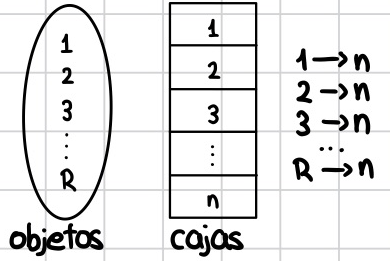
\includegraphics[width=\linewidth]{img-t2/img_035_24.png}
\end{wrapfigure}

Tenemos $r$ objetos diferentes en $n$ cajas diferentes (influye el orden). \textbf{VR(n, r)} = $n^r$ Es el número de aplicaciones de $r \xrightarrow{} n$ \\
Restricciones:
\begin{itemize}
    \item Todas las cajas deben tener 1 objeto (no estar vacías), por lo que $r \geq n$: es equivalente a contar el número de aplicaciones sobreyectivas de $r \xrightarrow{} n$.
    
    \item Como máximo hay 1 objeto en cada caja, por lo que $n \geq r$: es equivalente a contar el número de aplicaciones inyectivas de $r \xrightarrow{} n$, es decir \textbf{V(n, r)}.
\end{itemize}

\newpage

\subsection{Distribución de objetos iguales en cajas diferentes}

\begin{wrapfigure}[]{r}{0.3\linewidth}
    \centering
    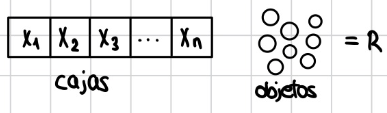
\includegraphics[width=\linewidth]{img-t2/img_603_36.png}
\end{wrapfigure}

Tenemos $r$ objetos iguales en $n$ cajas diferentes (no influye el orden). \textbf{CR(n, r)}. \\
Restricciones:
\begin{itemize}
    \item Todas las cajas deben tener 1 objeto (no estar vacías): es equivalente a contar el número de aplicaciones sobreyectivas de $r \xrightarrow{} n$ ($r \geq n$).

    \item Como máximo hay 1 objeto en cada caja, por lo que $n \geq r$: es equivalente a contar el número de cadeas de bits con $r$ unos, es decir, \textbf{C(n, r)}.
\end{itemize}

\section{Permutaciones con repetición}
Disponemos de $r$ tipos de objetos con la condición de que los objetos del mismo tipo son iguales entre sí y diferentes de los de otros tipos:
\begin{itemize}
    \item $n_1$ objetos del tipo 1 
    \item $n_2$ objetos del tipo 2
    \item ...
    \item $n_r$ objetos del tipo $r$
\end{itemize}

Tal que $n_1 + n_2 + ... + n_r = n$, las distintas permutaciones que se pueden  hacer de los $n$ objetos, se llamas \textbf{permutaciones con repetición de n objeetos con $n_1, n_2, ..., n_r$ repeticiones}. 
$$PR(n) = \frac{n!}{n_1!, n_2!, ..., n_r!}$$
(coeficiente multinomial, si $r$ = 2 coincide con el binomial y es igual a C(n, r)) \\

\textbf{Ejemplo}: ¿Cuántas palabras diferentes se pueden hacer con las letas de la palabra 'CASACA'? \\

$C_1, A_1, S_1, A_2, C_2, A_3$ (3 As, 2 Cs y una S): $PR(n) = \frac{6!}{3! \cdot 2! \cdot 1!}$

\newpage

\section{Coeficiente binomial y multinomial}
\subsection{Binomio de Newton}
\textbf{Se emplea para calcular los desarrollos de las expresiones $(a+b)^n$}. \\
$[(a+b)^3 = a^3 + 3a^2b + 3ab^2 + b^3]$ Nos basamos en contar el número de veces que aparece en una expresión los diferentes conjuntos. En $(a+b)^3$ aparece 1 vez el conjunto $\{aaa\}$ C(3, 3), 3 veces el conjunto $\{aab\}$ C(3, 2) y así con todos los conjuntos posibles. De esta manera se llega a la siguiente fórmula:
$$(a+b)^n = \sum_{k=0}^{n} \binom{n}{k} \cdot a^k \cdot b^{n-k} = \sum_{k=0}^{n} \binom{n}{k} \cdot a^{n-k} \cdot b^{k} $$ 

\textbf{Ejemplo}: ¿Cuál es el coeficiente de $x^{12}y^{13}$ en la expansión de $(2x-3y)^{25}$?
$$(2x-3y)^{25} = (2x+(-3y))^{25}$$
$$(2x+(-3y))^{25} = \sum_{j=0}^{25} \binom{25}{j}(2x)^{25-j}(-3y)^j$$
Por lo tanto, el coeficiente de $x^{12}y^{13}$ en la expansión es obtenido cuando $j = 13$: 
$$\binom{25}{13}2^{12}(-3)^{13} = -\frac{25!}{13!12!}2^{12}3^{13}$$.

Corolarios útiles: 
\begin{itemize}
    \item Sea $n$ un entero no negativo: $\sum_{k=0}^n \binom{n}{k} = 2^n$.

    \item Sea $n$ un entero no negativo: $\sum_{k=0}^n (-1)^k \binom{n}{k} = 0$.

    \item Sea $n$ un entero no negativo: $\sum_{k=0}^n 2^k \binom{n}{k} = 3^n.$
\end{itemize}

\subsection{Multinomio de Leibniz}


El \textbf{Multinomio de Leibniz} es una generalización del teorema del binomio de Newton, que permite expandir la potencia de la suma de varios términos. En lugar de solo dos términos $a + b$, se consideran $k$ términos.

\textbf{Fórmula general}: \\

La expansión de la expresión $(x_1 + x_2 + \dots + x_k)^n$ está dada por:

\[
(x_1 + x_2 + \dots + x_k)^n = \sum_{n_1 + n_2 + \dots + n_k = n} 
\binom{n}{n_1, n_2, \dots, n_k} x_1^{n_1} x_2^{n_2} \cdots x_k^{n_k},
\]

donde:

\[
\binom{n}{n_1, n_2, \dots, n_k} = \frac{n!}{n_1! \, n_2! \, \dots \, n_k!}
\]

\textbf{Condición:} La suma de los exponentes debe ser igual a $n$, es decir, $n_1 + n_2 + \dots + n_k = n$. 

\newpage

\textbf{Ejemplo}:

Expandamos \( (x_1 + x_2 + x_3)^4 \) usando el teorema del multinomio. Aquí \( n = 4 \) y \( k = 3 \).

\begin{itemize}
    \item Los posibles valores de \( n_1, n_2, n_3 \) que satisfacen \( n_1 + n_2 + n_3 = 4 \) son:
    \[
    (4, 0, 0), \, (3, 1, 0), \, (3, 0, 1), \, (2, 2, 0), \, (2, 1, 1), \, (2, 0, 2), \, (1, 3, 0), \, (1, 2, 1), \, (1, 1, 2), \, (1, 0, 3), \, (0, 4, 0), ...
    \]
\end{itemize}

Aplicando la fórmula del coeficiente multinomial:

\[
\binom{4}{n_1, n_2, n_3} = \frac{4!}{n_1! \, n_2! \, n_3!},
\]

calculamos los coeficientes para algunos términos:

\begin{align*}
\binom{4}{4, 0, 0} &= \frac{4!}{4! \, 0! \, 0!} = 1, \\
\binom{4}{3, 1, 0} &= \frac{4!}{3! \, 1! \, 0!} = 4, \\
\binom{4}{2, 2, 0} &= \frac{4!}{2! \, 2! \, 0!} = 6, \\
\binom{4}{1, 1, 2} &= \frac{4!}{1! \, 1! \, 2!} = 12, \\
\binom{4}{0, 0, 4} &= \frac{4!}{0! \, 0! \, 4!} = 1.
\end{align*}

Por lo tanto, la expansión completa es:

\begin{equation}
\begin{aligned}
(x_1 + x_2 + x_3)^4 &= x_1^4 + 4x_1^3 x_2 + 4x_1^3 x_3 \\
&\quad + 6x_1^2 x_2^2 + 12x_1^2 x_2 x_3 + 6x_1^2 x_3^2 \\
&\quad + 4x_1 x_2^3 + 12x_1 x_2^2 x_3 + 12x_1 x_2 x_3^2 \\
&\quad + 4x_1 x_3^3 + x_2^4 + 4x_2^3 x_3 \\
&\quad + 6x_2^2 x_3^2 + 4x_2 x_3^3 + x_3^4.
\end{aligned}
\end{equation}

\newpage

\section{Identidad de Pascal}
Sean $n$ y $k$ positivos entero con $n \geq k$. Entonces 
$$\binom{n+1}{k} = \binom{n}{k-1} + \binom{n}{k}.$$
Esta igualdad se deduce de sumar los subconjuntos de $k$ elementos que contienen al elemento $a_2$ $C(n-1, k-1)$ y los que no $C(n-1, k)$, que da el número de subconjuntos de $k$ elementos $C(n, k)$. Este triángulo sirve para calcular número combinatorios, binomios de Newton o el número de elementos de partes de un conjunto de n elementos (suma de la fila $n$).

\begin{figure}[h]
    \centering
    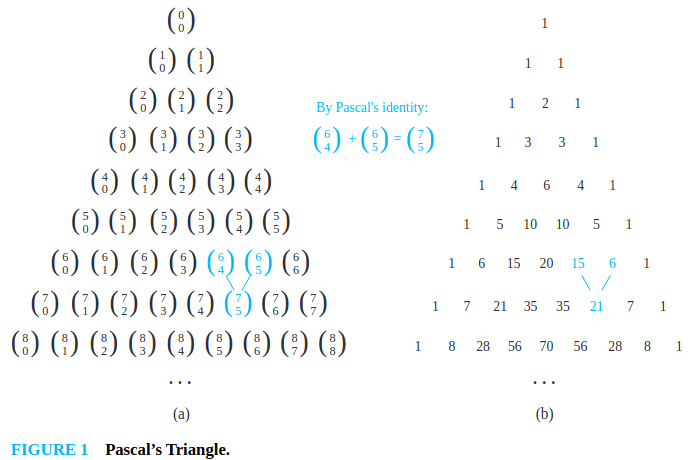
\includegraphics[width=0.7\textwidth]{img-t2/img_881_04.png}
\end{figure}

\newpage

\section{Principio de inclusión-exclusión}
\textbf{Sean $A$ y $B$ dos conjuntos no disjuntos $|A \cup B| = |A| + |B-A| = |A| + |B| - |A \cap B|$}. \\
Sean $C_1, C_2, ..., C_n$ un número finito de conjuntos:

$$|C_1 \cup C_2 \cup ... \cup C_n| = \sum_{1 \leq i \leq n}^n |C_i| 
- \sum_{1 \leq i \leq j \leq n} |C_i \cap C_j| 
+ \sum_{1 \leq i \leq j \leq k \leq n} |C_i \cap C_j \cap C_k|
- ... + (-1)^{n+1} \cdot |C_1 \cap C_2 \cap ... \cap C_n|$$

\textbf{Ejemplo}: Un total de 1232 estudiantes han tomado un curso de español, 879 han tomado un curso de francés y 114 han tomado un curso de ruso. Además, 103 han tomado cursos de español y francés, 23 han tomado cursos de español y ruso, y 14 han tomado cursos de francés y ruso. Si 2092 estudiantes han tomado al menos uno de los cursos de español, francés y ruso, ¿cuántos estudiantes han tomado un curso en los tres idiomas? \\

Sea $S$ el conjunto de estudiantes que han tomado un curso de español, $F$ el conjunto de estudiantes que han tomado un curso de francés y $R$ el conjunto de estudiantes que han tomado un curso de ruso. Entonces: \\
$|S| = 1232,$ $|F| = 879,$ $|R| = 114,$ $|S \cap F| = 103,$ $|S \cap R| = 23,$ $|F \cap R| = 14,$ y $|S \cup F \cup R| = 2092$. 

$$|S \cup F \cup R| = |S| + |F| + |R| - |S \cap F| - |S \cap R| - |F \cap R| + |S \cap F \cap R|$$

$$2092 = 1232 + 879 + 114 - 103 - 23 - 14 + |S \cap F \cap R|$$

$$|S \cap F \cap R| = 7$$

\begin{figure}[h]
    \centering
    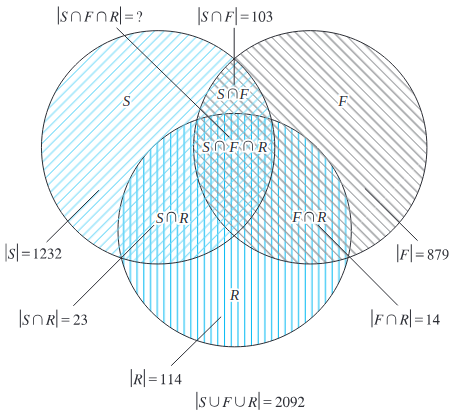
\includegraphics[width=0.65\textwidth]{img-t2/img_287_39.png}
\end{figure}

\newpage

\section{Numeración de aplicaciones sobreyectivas entre conjuntos}
Tengamos un conjunto de $r$ elementos y otro de $n$ elementos ($r \geq n$). Debemos \textbf{distribuir $r$ objetos diferentes en $n$ cajas diferentes sin que haya cajas vacías}. \\
Sea $C_i$ una caja, ninguna puede quedar vacía. \\
En el caso que $r = 6$, $n = 4$:

$$|\overline{C_1} \cap \overline{C_2} \cap \overline{C_3} \cap \overline{C_4}| = |\overline{C_1 \cup C_2 \cup C_3 \cup C_4}| = |U - (C_1 \cup C_2 \cup C_3 \cup C_4)| = |U| - |C_1 \cup C_2 \cup C_3 \cup C_4)|$$
El número de elementos de U es VR(n, r) y el del segundo término (con el principio de inclusión-exclusión) es $C(4, 1) \cdot 3^6 - C(4, 2) \cdot 2^6 + C(4, 3) \cdot 1^6 - C(4, 4) \cdot 0^6$. \\
Así, nos queda \textbf{la expresión}:
$$\sum_{k=0}^n (-1)^k \cdot \binom{n}{k} \cdot (n-k)^r$$




\begin{comment}
\begin{figure}[h]
    \centering
    \includegraphics[width=0.65\textwidth]{1.png}
    \caption{}
\end{figure}
\end{comment}

\begin{comment}
\begin{wrapfigure}[]{r}{0.45\linewidth}
    \centering
    \includegraphics[width=0.8\linewidth]{8.png}
    \caption{}
\end{wrapfigure}
\end{comment}

\end{document}